\documentclass[hyperref={pdfpagelayout=SinglePage},10pt]{beamer}\usetheme{Antibes}\usepackage{euler}\usepackage{pgf}
\usecolortheme{whale}
\useoutertheme{infolines}\usepackage{epstopdf}\usepackage{xcolor}\usepackage{multicol}

\usepackage{float}
%\RequirePackage[colorlinks,breaklinks]{hyperref}
\hypersetup{linkcolor=blue,citecolor=blue,filecolor=black,urlcolor=blue}

\definecolor{utorange}{RGB}{191,87,0}
%\useinnertheme{default}
\usefonttheme{serif}
\usepackage{palatino}
\beamertemplatenavigationsymbolsempty
\setbeamerfont{title like}{shape=\scshape}

%\setbeamerfont{frametitle}{shape=\scshape}
%\setbeamercolor*{frametitle}{fg=utorange,bg=white}
%\setbeamercolor*{section in head/foot}{bg=white,fg=utorange}
%\setbeamercolor*{normal text}{fg=black,bg=white}
%\setbeamercolor*{structure}{fg=black}
\setbeamertemplate{footline}

\setbeamertemplate{footline}
{ 
    \leavevmode%
    \hbox{%
        \begin{beamercolorbox}[wd=.333333\paperwidth,ht=2.25ex,dp=1ex,center]{section in head/foot}%
            \usebeamerfont{author in head/foot}{Aaron Webb}
        \end{beamercolorbox}%
        \begin{beamercolorbox}[wd=.333333\paperwidth,ht=2.25ex,dp=1ex,center]{section in head/foot}%
            \usebeamerfont{title in head/foot}{Gradient Boosted Decision Trees in Particle Physics}%\insertshorttitle
        \end{beamercolorbox}%
        \begin{beamercolorbox}[wd=.333333\paperwidth,ht=2.25ex,dp=1ex,right]{section in head/foot}%
            \usebeamerfont{date in head/foot}\insertshortdate{}\hspace*{2em}
            \insertframenumber{} / \inserttotalframenumber\hspace*{2ex} 
        \end{beamercolorbox}}%
        \vskip0pt%
    }
    \makeatother

\def\tth{\ensuremath{t\bar{t}H}}

\renewcommand{\(}{\begin{columns}}
\renewcommand{\)}{\end{columns}}
\newcommand{\<}[1]{\begin{column}{#1}}
\renewcommand{\>}{\end{column}}

\author{\large Aaron Webb}
\date{October 27, 2017}


\title{\huge Gradient Boosted Decision Trees and Particle Physics}

\begin{document}

\frame{\titlepage}

\frame{\frametitle{The LHC and Big Data}\tiny

    \begin{itemize}\large
        \item Bunches of $10^{11}$ protons are collided every 25 ns
        \item Produces $\approx$ 50 PB of data per year
        \item Particle lifetimes $\mathcal{O}(10^{-25})$ seconds, only ever see decay products
    \end{itemize}

\begin{columns}[T]
    \begin{column}{0.43\textwidth}
    \begin{itemize}\large
        \item Many processes look the same in the detector
        \item Interesting interactions are rare
    \end{itemize}
    \end{column}
    \begin{column}{0.55\textwidth}
    \begin{figure}
        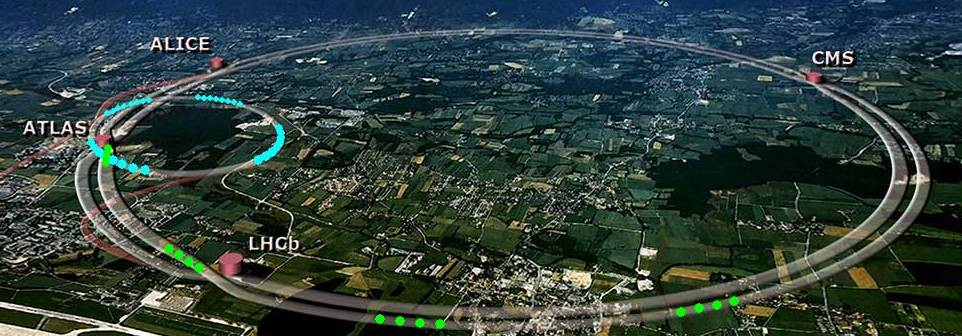
\includegraphics[width=0.95\textwidth]{lhc-aerial.jpg}
    \end{figure}
    \end{column}
\end{columns}
}


\frame{\frametitle{The ATLAS Dectector}

\begin{columns}[T]
    \begin{column}{0.3\textwidth}
    \begin{itemize}\large
        \item Tells us the types of particles, their momentum, energy, and location
        \item Use these to predict what happened  
    \end{itemize}
    \end{column}
    \begin{column}{0.75\textwidth}
    \begin{figure}
        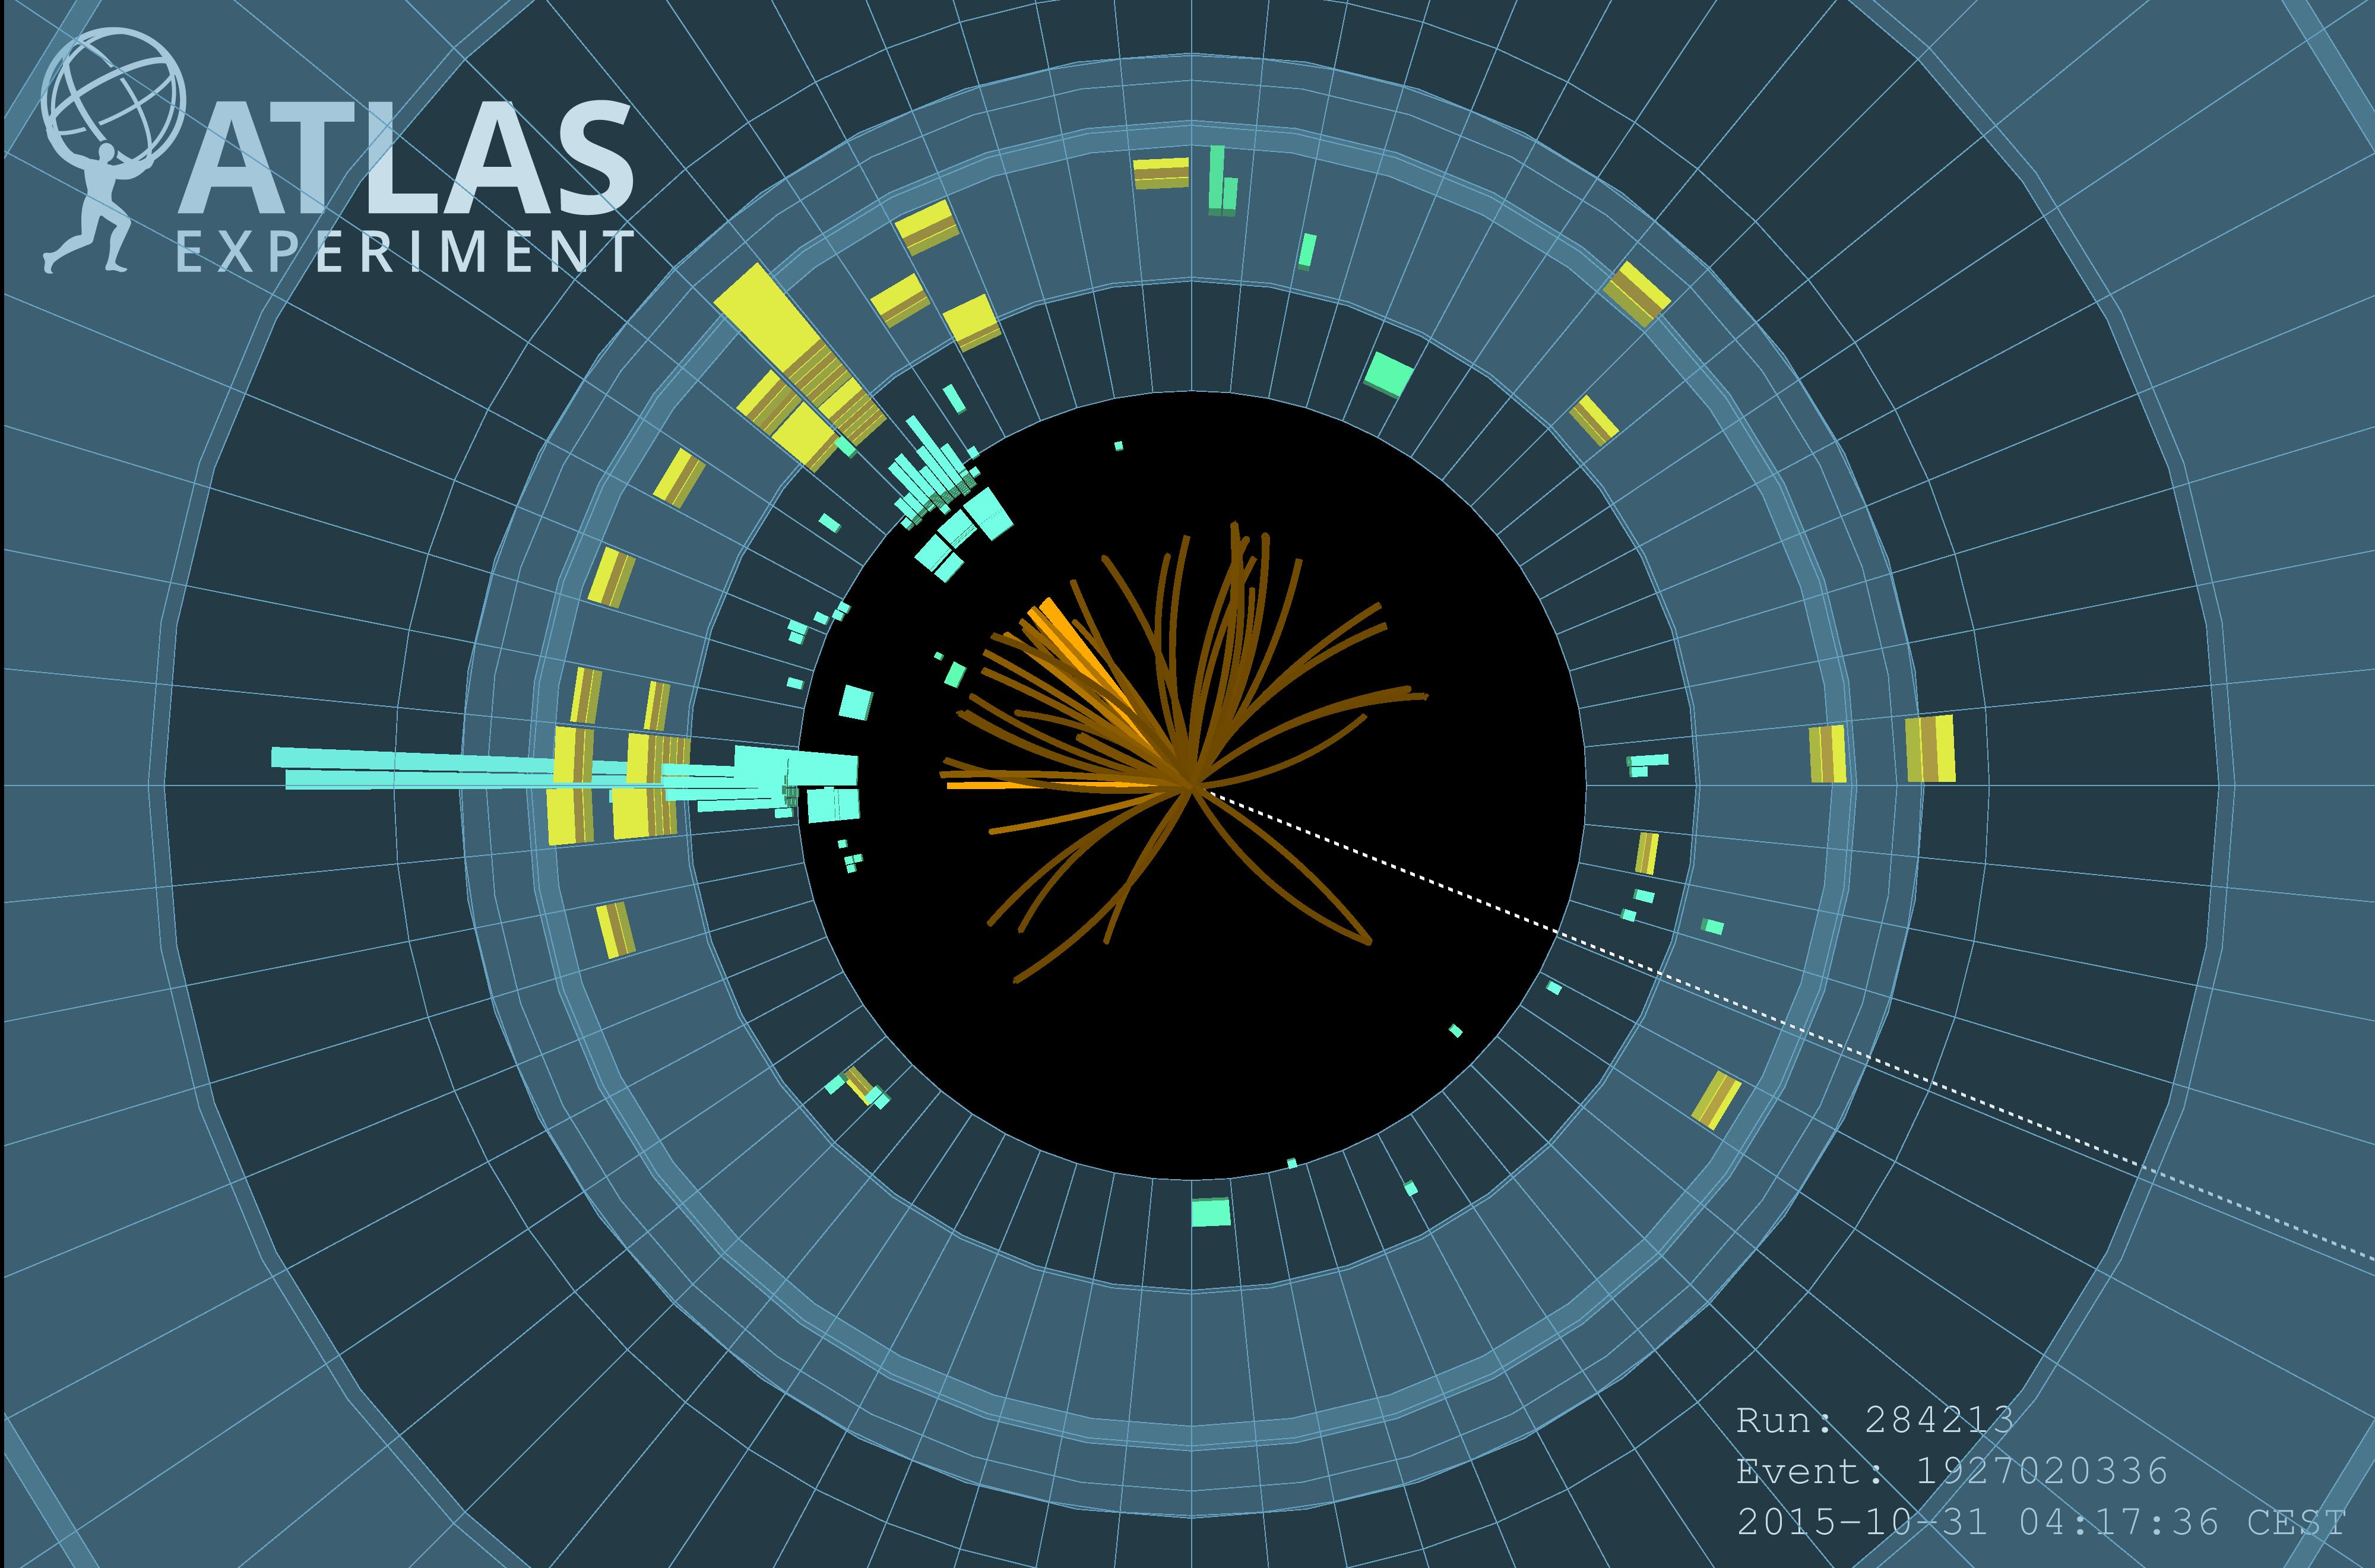
\includegraphics[width=0.95\textwidth]{event_display.png}
    \end{figure}
    \end{column}
\end{columns}

}

\frame{\frametitle{Gradient Boosted Decision Trees}

    \begin{columns}[T]
    \begin{column}{0.5\textwidth}

    \begin{itemize}
        \item Combines a set of weak "learners" into a single "strong" learner
        \item Start with a simple model - single binary decision tree
        \item Construct a new tree to correct the weaknesses of the model
        \item Iterate till it converges
    \end{itemize}
    
    \end{column}
    \begin{column}{0.5\textwidth}
    \begin{figure}
        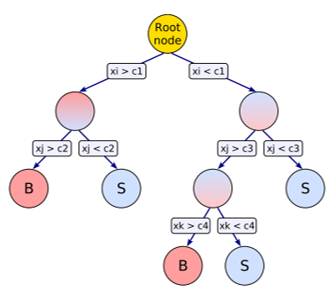
\includegraphics[width=0.95\textwidth]{bdt_tree.png}
    \end{figure}
    \end{column}
\end{columns}

}

\frame{\frametitle{The Algorithm}

\begin{itemize}
    \item Create a model, $F(x)$, for a data set y
    \item Start with a simple model, $F_0(x) = \underset{\gamma}{\arg\min} \sum_{i=1}^n L(y_i, \gamma)$
    \item Model the residuals: $h(x) = y - F_0(x)$
    \item Update the model: $F_{m+1}(x)=F_{m}(x)+h(x)$
    \item Iterate till the model converges
    \item $F(x)=\sum _{{i=1}}^{M}\gamma _{i}h_{i}(x)+{\mbox{const}}$
\end{itemize}

}

\frame{\frametitle{Improvements}
    \begin{itemize}
        \item Shrinkage 
        \begin{itemize}
            \item $F_m(x) = F_{m-1}(x) + \nu \cdot \gamma_m h_m(x), \quad 0 < \nu \leq 1$
            \item $\nu$ is the "learning rate", typically $<$0.1
            \item Improves results, but increases computation costs
        \end{itemize}
        \item Stochastic Boosting
        \begin{itemize}
            \item Each successive tree is fit to a random subsample
            \item Prevents overfitting, improves speed
        \end{itemize}
        \item $l_2$ penalty term
        \begin{itemize}
            \item Penalize complex trees, remove branches that produce no differentiation
        \end{itemize}
    \end{itemize}
}

\frame{\frametitle{Pros and Cons}
    
    \begin{columns}[T]
    \begin{column}{0.5\textwidth}
    
    Pros
    \begin{itemize}
        \item Easy to use once model has been developed
        \item Few input parameters needed to tune
        \item General framework, relevant for a large number of applications
    \end{itemize}
    \end{column}
    
    \begin{column}{0.5\textwidth}

    Cons
    \begin{itemize}
        \item Training the model can be slow
        \item Difficult to interpret the output
        \item Not ideal for sparse data, large numbers of features
    \end{itemize}
    \end{column}
\end{columns}

}

\frame{\frametitle{Uses in Particle Physics}

\begin{columns}[T]
    \begin{column}{0.55\textwidth}
    \begin{itemize}\large
        \item Separate signal and background events
        \begin{itemize}
            \item Use Monte Carlo simulations to train the model, use for data
        \end{itemize}
        \item Distinguish "real" particles from "fakes"
        \begin{itemize}
            \item Particles misidentified by the detector, from secondary sources
        \end{itemize}
        \item "B-tagging" - identifying different flavors of quarks
        \begin{itemize}
            \item Quarks "hadronize", leaving complex signatures 
        \end{itemize}
    \end{itemize}
    \end{column}
    \begin{column}{0.45\textwidth}
    \begin{figure}
        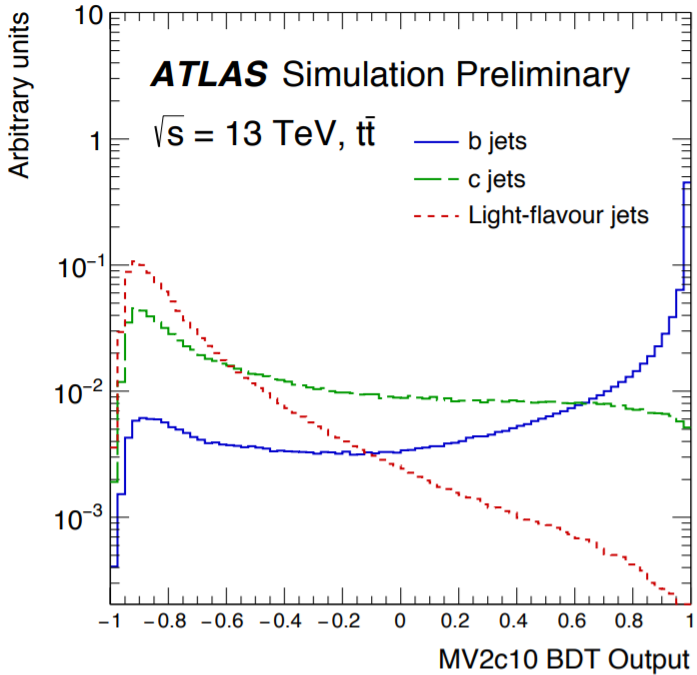
\includegraphics[width=0.95\textwidth]{MV2c10_output.PNG}
    \end{figure}
    \end{column}
\end{columns}

}

\frame{\frametitle{Vector Boson Scattering}
        
\begin{columns}[T]
    
    \begin{column}{0.45\textwidth}
    \begin{figure}
        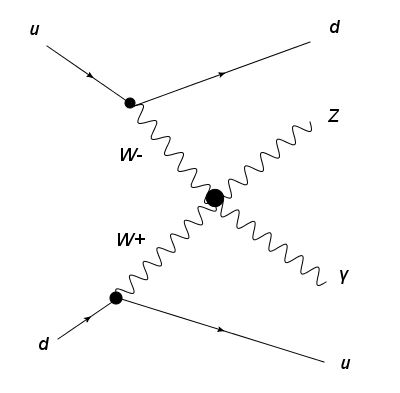
\includegraphics[width=0.95\textwidth]{VBSdiagram.JPG}
    \end{figure}
    \end{column}
    
    \begin{column}{0.45\textwidth}
    \begin{figure}
        \centering
        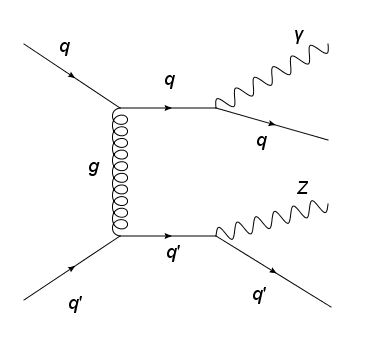
\includegraphics[width=0.95\textwidth]{QCD_Zg.JPG}
    \end{figure}
    \end{column}
    
\end{columns}
}

\frame{\frametitle{Results}

\begin{columns}[T]
    

    \begin{column}{0.25\textwidth}
    \begin{figure}
        \centering
        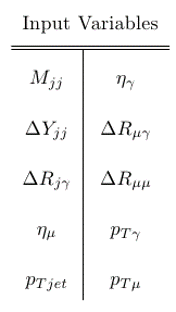
\includegraphics[width=0.9\textwidth]{input_var.png}
    \end{figure}
    \end{column}
    
    \begin{column}{0.75\textwidth}
    \begin{figure}
        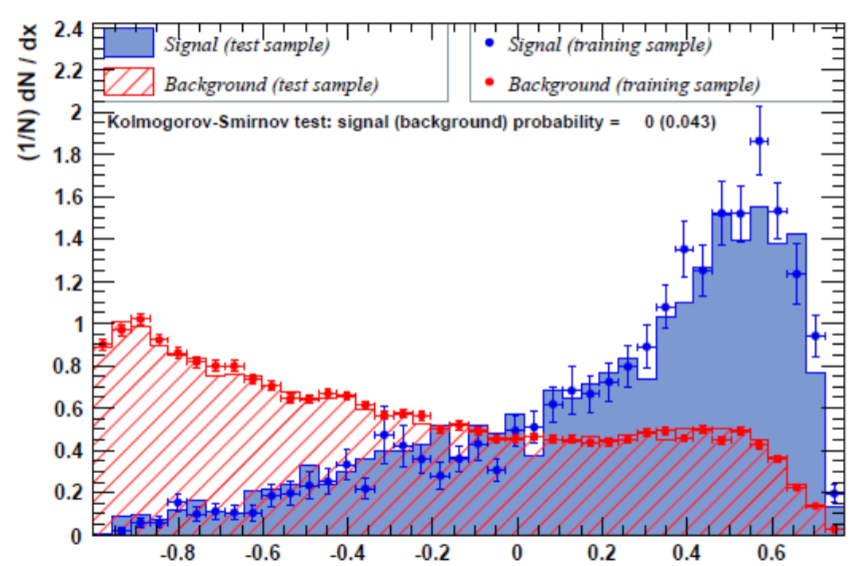
\includegraphics[width=0.95\textwidth]{bdt_response.PNG}
    \end{figure}
    \end{column}
    
\end{columns}

}

\frame{\frametitle{Results}
    \begin{figure}
        \centering
        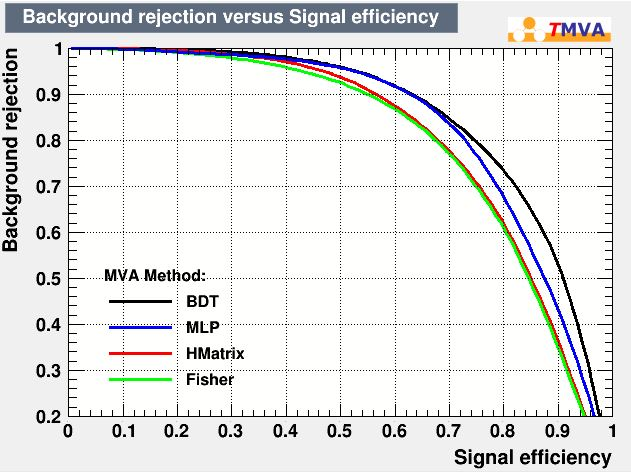
\includegraphics[width=0.75\textwidth]{ROC_curve.JPG}
    \end{figure}
}
\end{document}